\documentclass[10pt,a4paper]{article}
\usepackage[utf8]{inputenc}
\usepackage{lmodern}
\usepackage[T1]{fontenc}
\usepackage[brazil]{babel}
\usepackage{amsmath}
\usepackage{amsfonts}
\usepackage{amssymb}

\usepackage{float}         % For positioning images
\usepackage{graphicx}      % For image support
\graphicspath{ {images/} } % Store images in a different directory

\usepackage{titlesec}      % Customize section titles
\titleformat{\section}{\bf}{\thesection.}{5pt}{\bf}
\titleformat{\subsection}{\bf}{\thesubsection.}{5pt}{\bf}

\usepackage{indentfirst}   % Add first line indent
\usepackage{booktabs}      % Table decoration

% Table Hacks
% https://tex.stackexchange.com
% /questions/192842/multiple-columns-in-table-problem-with-alignment
\usepackage{array}
\newcolumntype{L}[1]{
    >{\raggedright\let\newline\\\arraybackslash\hspace{0pt}}p{#1}
}
\newcolumntype{C}[1]{
    >{\centering\let\newline\\\arraybackslash\hspace{0pt}}p{#1}
}
\newcolumntype{R}[1]{
    >{\raggedleft\let\newline\\\arraybackslash\hspace{0pt}}p{#1}
}

\author{Ariel Nogueira Kovaljski}
\title{Trabalho de Linguagens Formais e Autômatos}
\date{<dia-atual> de maio de 2021}

\begin{document}
    \begin{center}
    \makeatletter

    \LARGE
    \@title

    \vspace{0.5cm}

    \large
    \@author \\
    \small
    \texttt{<arielnogueirak@gmail.com>}


    \vspace{0.5cm}

    \normalsize
    \textit{
       Computer Engineering Course, \\
       Instituto Politécnico (IPRJ) --- Rio de Janeiro State University, \\
       Rua Bonfim 25, Nova Friburgo, RJ 28625-570, Brazil
    }

    \vspace{0.5cm}
    \@date

    \makeatother
    \vspace{0.5cm}
    \hrule
\end{center}

\section*{Abstract}

In this article we build and analyze the behavior and output of a Finite State
Machine (FSM) and a Turing Machine (TM) for a given set of inputs.

\medskip
\noindent
\textit{Keywords:} finite state machine, turing machine, finite automata

\section*{Resumo}

Neste artigo nós construímos e analisamos o comportamento e a saída de uma
Máquina de Estado Finito (MEF) e uma Máquina de Turing (MT) para um dado
conjunto de entradas.

\medskip
\noindent
\textit{Palavras-chave:} máquina de estado finito, máquina de turing, autômatos
finitos
    \section{Introdução}

A teoria de autômatos trata do estudo de máquinas abstratas que seguem
instruções pré-determinadas automaticamente.

<falar sobre níveis da hierarquia de chomsky>

A partir da hierarquia de Chomsky de gramáticas formais, é possível definir
autômatos que são capazes de reconhecer linguagens formais pertencentes a
distintas classes de gramática. Sendo assim, para uma linguagem formal
possivelmente infinita, define-se um autômato como uma representação finita
desta linguagem.

\begin{figure}[H]
    \centering
    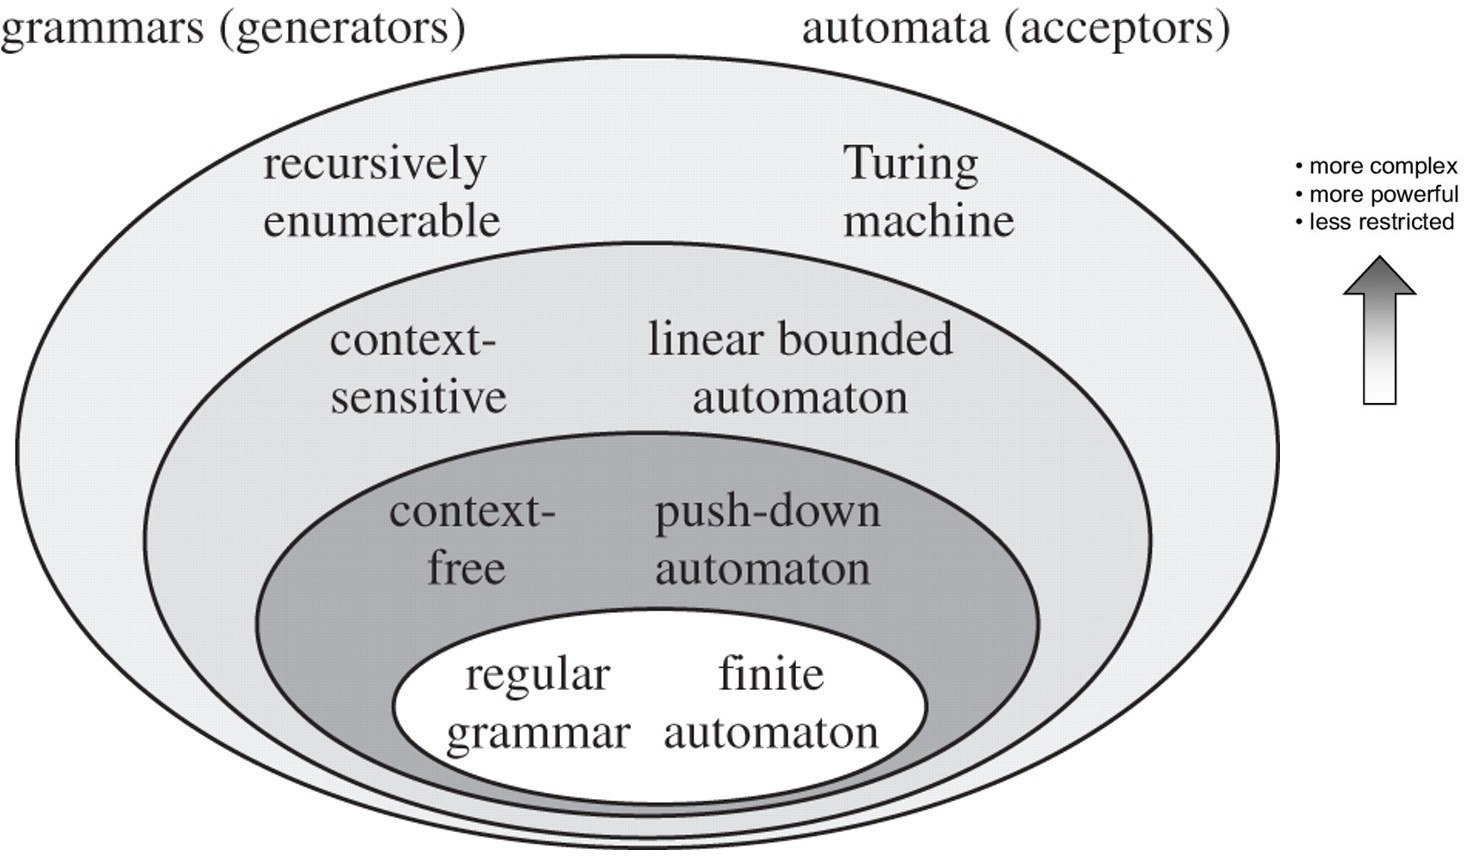
\includegraphics[width=0.8\textwidth]{chomsky}
    \label{chomsky}
    \caption{Hierarquia de Chomsky}
\end{figure}

Dentre os tipos de autômatos existentes, neste trabalho iremos abordar a
construção e o funcionamento das \emph{máquinas de estado finito} e das
\emph{máquinas de Turing}. Estes são responsáveis pelo reconhecimento das
\emph{gramáticas regulares } e \emph{recusivamente enumeráveis},
respectivamente.

    \section{Desenvolvimento}

Iremos nos aprofundar no desenvolvimento destes autômatos. <expandir>

\subsection{Máquina de Estado Finito}

<falar sobre memória>

Uma máquina de estado finito (MEF) pode ser considerada como um modelo
simplificado do funcionamento de um computador. Esta pode ser definida como uma
quíntupla ordenada $M = (S, I, O, f_S, f_O)$ onde:
\begin{itemize}
    \item $S$ é o conjunto finito de estados;
    \item $I$ é o conjunto finito de símbolos de entrada (alfabeto de entrada);
    \item $O$ é o conjunto finito de símbolos de saída (alfabeto de saída);
    \item $f_S: S \times I \rightarrow S$ é uma função que retorna o próximo
          estado $s_{t_{k+1}} \in S$ dado o estado anterior $s_{t_k} \in S$ e
          um símbolo de entrada $i_{t_k} \in I$;
    \item $f_O: S \rightarrow O$ é a função \textit{output}, que retorna o
          símbolo de saída $o_{t_k} \in O$ do estado atual $s_{t_k} \in S$.
\end{itemize}

As operações da MEF são sincronizadas por pulsos discretos de um relógio
(\emph{clock}) representados por $t_k$, onde $k \in \mathbb{N}_0$ representa o
ciclo de \textit{clock} atual. Partindo de um estado inicial $s_0 = s_{t_0}$,
após um pulso de \textit{clock}, a função $f_S$ retornará um novo estado
$s_{t_1}$ dado a entrada anterior $i_{t_0}$ e o estado anterior $s_0$.
Generalizando para qualquer pulso de \textit{clock}, é possível afirmar que a
MEF possui um comportamento determinístico, ou seja, o novo estado sempre
dependará do estado e entrada anteriores. Para cada um dos estados, há um
símbolo de saída, que é retornado pela função \textit{output} $f_O$.

\begin{figure}[H]
    \centering
    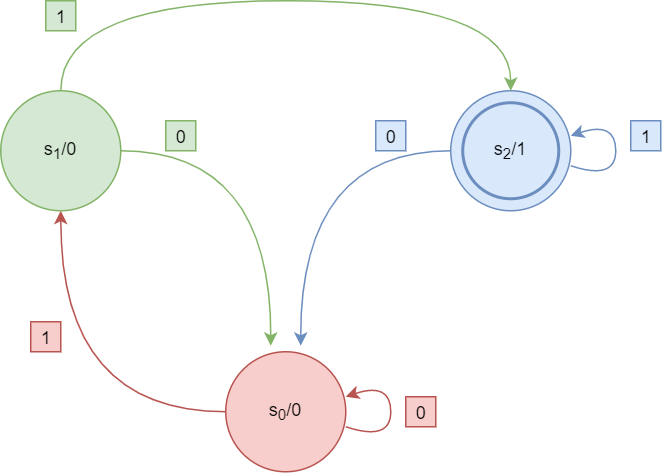
\includegraphics[width=0.7\textwidth]{fsm}
    \caption{Exemplo de máquina de estado finito}
\end{figure}

Tomando como exemplo a MEF acima, começamos no estado $s_0$ e temos como saída o
símbolo \textbf{0}. Aqui, há duas possibilidades: enquanto a entrada for
\textbf{0}, permanecemos neste estado; caso a entrada seja \textbf{1}, seguimos
para o estado $s_1$. Ao seguirmos para o estado $s_1$ temos como saída o símbolo
\textbf{0}. Novamente, há duas possíveis entradas: caso a entrada seja
\textbf{0}, retornamos ao estado $s_0$; caso a entrada seja \textbf{1}, seguimos
para o estado $s_2$. Por fim, ao seguirmos para o estado $s_2$ temos como saída
o símbolo \textbf{1}. As alternativas são: caso a entrada seja \textbf{0},
retornarmos ao estado $s_0$; enquanto a entrada seja \textbf{1}, permanecemos
neste estado.

Esta forma um tanto verbosa de se descrever uma MEF pode ser colocada em uma
tabela, com o estado atual, possíveis entradas e saídas como colunas da mesma.

\begin{center}
    % https://tex.stackexchange.com
    % /questions/192842/multiple-columns-in-table-problem-with-alignment
    % Use `L{width}', `C{width}' or `R{width}' for column alignment
    \begin{tabular}{ c C{1cm} C{1cm} c }
        \toprule
        Estado Atual & \multicolumn{2}{c}{Próximo Estado} & Saída  \\
                     & \textbf{0} & \textbf{1} &                   \\
        \hline
        $s_0$        & $s_0$      & $s_1$      & \textbf{0}        \\
        $s_1$        & $s_0$      & $s_2$      & \textbf{0}        \\
        $s_2$        & $s_0$      & $s_2$      & \textbf{1}        \\
        \bottomrule
    \end{tabular}
\end{center}

Nota-se que dentre todas as possíveis entradas, esta MEF só aceitará, isto é,
terminará no estado final $s_2$, para \emph{strings} de entrada que terminem
com dois ou mais \textbf{1} (\textbf{11}, \textbf{111}, \textbf{1111}, \ldots).

\subsection{Máquina de Turing}

<expandir>
    \section{Conclusão}

A teoria das linguagens formais e autômatos é fundamental no ramo da
computação. Dentre as suas aplicações, encontram-se análise sintática,
compiladores, inteligência artificial, verificação formal e muitas outras.

Através da construção e execução de máquinas de estado finito e máquinas de
Turing, foi possível melhor entender a teoria por trás de seu funcionamento,
suas aplicações, e em quais situações se deve preferir o uso de uma ou da outra.
    \section{Referências Bibliográficas}

\textbf{Figura \ref{chomsky}:} Fitch, Tecumseh. 2014. \textit{``Toward a
computational framework for cognitive biology: Unifying approaches from
cognitive neuroscience and comparative cognition''}
\end{document}
